\scanpage{2}
% cote 123
Compléments sur transformation de Coxeter d'un système de racines\inserted{\handwritten{
\begin{tikzpicture}[baseline=(word.base),x=1cm,y=1cm]
\node[inner sep=1pt] (word) at (0,0) {\unsure{irréductible|irreductible}};
\draw (0,0) ellipse (1.15 and 0.24);
\draw (-0.6,-0.2) .. controls (-0.4,-0.34) and (-0.64,-0.43) .. (-0.59,-0.62);
\end{tikzpicture}}} (Kostant).
% Handwritten reference below the title, extending across the page.
\par\noindent\hspace*{1.6cm}\handwritten{The principal 3-dimensional subgroup ....\quad th. 9.2.}\par

a) Soit $w\handwritten{\in}W$. Alors toute valeur propre de $w$ \unsure{est} une racine de $1$ d'ordre divisant un des entiers $m_i+1$ (où les $m_i$ sont les exposants caractéristiques), donc d'ordre $\handwritten{\leq}h$. Pour qu'il y en ait une qui soit d'ordre $h$, il faut et suffit que $w$ soit une transformation de Coxeter, et\inserted{alors} les éléments non nuls du sous-espace propre correspondant\inserted{\handwritten{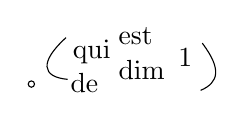
\begin{tikzpicture}[baseline=(qui.base),x=1cm,y=1cm]
\node[anchor=base west,inner sep=0pt] (qui) at (0,0) {qui};
\node[anchor=base west,inner sep=0pt] at (0.58,0.18) {est};
\node[anchor=base west,inner sep=0pt] at (-0.03,-0.43) {de};
\node[anchor=base west,inner sep=0pt] at (0.58,-0.26) {dim};
\node[anchor=base west,inner sep=0pt] at (1.34,-0.1) {$1$};
\draw (-0.08,0.27) .. controls (-0.42,-0.04) and (-0.39,-0.23) .. (-0.06,-0.26);
\draw (1.65,0.2) .. controls (1.9,-0.13) and (1.86,-0.3) .. (1.63,-0.4);
\draw (-0.52,-0.32) circle (0.04);
\end{tikzpicture}}} sont des éléments réguliers.
% The preceding inserted note is in the left margin, with an open-circle call after « correspondant »; the internal stagger is retained.
\margin{\handwritten{\figure{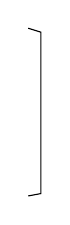
\begin{tikzpicture}[x=1cm,y=1cm]\draw (-0.16,0.05)--(0,0)--(0,-2.05)--(-0.16,-2.08);\end{tikzpicture}}}}

\uline{Corollaire}\handwritten{1}: Soit $\handwritten{\mu}$ le sous-groupe de $W$ engendré par un élément de Coxeter $c$, donc $\handwritten{\mu\simeq}\underline{Z}\handwritten{/}h\underline{Z}$. Alors $\handwritten{\mu}$ est égal au centralisateur de $c$, donc de $\handwritten{\mu}$, et si $\handwritten{\nu}$ est le normalisateur de $\handwritten{\mu}$, l'homomorphisme
\begingroup\reversemarginpar
\margin{\handwritten{\figure{\begin{tikzpicture}[x=1cm,y=1cm]\draw (0,0)--(0,-2.4);\end{tikzpicture}}}}
\endgroup
\[
\handwritten{\unsure{\nu|\psi}/\mu\longrightarrow}\operatorname{Aut}(\handwritten{\mu})\handwritten{\simeq}(\underline{Z}/h\underline{Z})^{\handwritten{*}}
\]
\margin{\handwritten{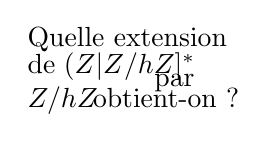
\begin{tikzpicture}[x=1cm,y=1cm]
\node[anchor=base west,inner sep=0pt] at (0,0) {Quelle extension};
\node[anchor=base west,inner sep=0pt] at (0,-0.34) {de};
\node[anchor=base west,inner sep=0pt] at (0.46,-0.34) {$(\unsure{\mathbb{Z}|Z}/h\mathbb{Z}]^*$};
\node[anchor=base west,inner sep=0pt] at (1.61,-0.5) {par};
\node[anchor=base west,inner sep=0pt] at (0,-0.77) {$\mathbb{Z}/h\mathbb{Z}$};
\node[anchor=base west,inner sep=0pt] at (0.83,-0.77) {obtient-on ?};
\end{tikzpicture}}}
est \unsure{un} isomorphisme; en d'autres termes, pour tout entier $n$ premier à $h$, il existe un $w\handwritten{\in}W$ tel que $wcw^{-1}=c^h$, et $w$ est déterminé mod $\handwritten{\mu}$.
\begingroup\reversemarginpar
% slanted
\margin{\handwritten{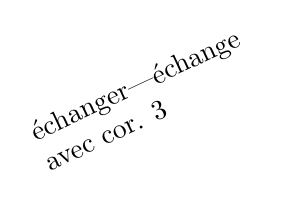
\begin{tikzpicture}\node[rotate=25,align=left,inner sep=0pt] {\unsure{échanger|échange}\\avec cor. 3};\end{tikzpicture}}}
\endgroup

Soit \unsure{en} ef\inserted{f}et $D$ \deleted{\unsure{une droite}}\inserted{le sous-espace} propre sous $c$ correspondant à une racine primitive $h$.ème de $1$. Alors $\dim D=1$ (prop.\handwritten{30}), et $\handwritten{\unsure{\mathfrak{z}|z}}=\operatorname{Centr}(\handwritten{\mu})$ normalise $D$, d'où un homomorphisme $\handwritten{\mathfrak{z}\to}\operatorname{Aut}(D)=\underline{C}^{\handwritten{*}}$, dont l'image est un sous-groupe fini de $\underline{C}^{\handwritten{*}}$, contenant l'image (isomorphe) de $\handwritten{\mu}$, donc cyclique d'ordre un multiple de $h$. Grâce à Kostant, son ordre est égal à $h$, et on a donc trouvé une rétraction $\handwritten{\mathfrak{z}\to\mu}$, il faut prouver que son noyau est réduit à $1$. Or si $w$ est dans ce noyau, il \deleted{induit} centralise $D$, et q\unsure{ô|ö}mme $D$ est régulière par Kostant,cela implique $w=1$. \unsure{Bn|On} a donc prouvé $\handwritten{\mathfrak{z}}=\handwritten{\mu}$. Reste à prouver que si $n$ est un entier premier à $h$, alors $c^n$ est conjugué de $c$, ce qui résulte également de Kostant.

\uline{Corollaire}. Soit $c$ un élément de Coxeter, et $\handwritten{\lambda}$ une valeur propre de $c$, correspondant à un vecteur propre $x$. Pour que $x$ soit régulier, il faut et il suffit que $\handwritten{\lambda}$ soit une racine primitive $h$.ème de $1$.
\begingroup\reversemarginpar
\margin{\handwritten{\figure{
\begin{tikzpicture}[x=1cm,y=1cm]\draw (0.05,0)--(0,-0.15)--(0,-1.05);\end{tikzpicture}}}}
\endgroup

La suffisance a déjà été énoncée avec le th. de Kostant. Pour la nécessité, soit $h'\handwritten{\leq}h$ l'ordre de la valeur propre, alors $c^{h'}$ centralise $x$, donc, $x$ étant régulier, on a $c^{h'}=1$, donc $h'=h$, cqfd.

\uline{Corollaire}. \deleted{\unsure{Considérons}} \deleted{Soit $D$ une}\inserted{Soit $D$ une} droite régulières dans $V\mathbin{\text{\textcircled{x}}}\underline{C}$ telle qu'il existe un élé%
% The physical line ends with a word-division hyphen; the word continues on the next scan.
% archive sheet number: 1
